\section{Crosscutting Concept}

In this chapter we will present the technical solutions that we will use to develop this project.
For each quality attribute we will present the chosen tactics.

\subsection{Solution for Usability}

The core of our app is how easy it is to use. We want our user to navigate through it without being overwhelmed with information
not related to the main objective: purchase a product or upload a product.

% \begin{table}[H]
%     \setstretch{1.0}
%     \begin{tabularx}{\textwidth}{|c|c|X|c|}
%         \toprule
%         \multicolumn{1}{c}{Tactict} & \multicolumn{1}{c}{Pattern} & \multicolumn{1}{c}{Motivation} & \multicolumn{1}{c}{QA} \\
%         \midrule
%         \textbf{Support User Initiative } & Observer & The interaction of the users is a main factor of our app.
%         We want them to have fully control of their actions either by cancelling or by resuming an action. & QA-1 \\
%         \textbf{Support User Initiative } & Lazy Registration & Avoid having to memorize another password and username
%         may increase the acceptance of the user. With this pattern we allow them also to browse in the app and seeing
%         what is available without being registered \cite{refonline:IDUI}. This may give a glimpse of what they get
%         if they join us. & QA-1 \\
%         \textbf{Support System Initiative} & Observer & By each upload from the \glsplural{provider} we want our
%         \glsplural{client} to have it on his device, without having to "ask" for it. & QA-1  \\
%         \bottomrule
%     \end{tabularx}
% \end{table}


% Please add the following required packages to your document preamble:
% \usepackage{booktabs}
% \usepackage{multirow}
% \usepackage{graphicx}
\begin{table}[H]
    \setstretch{1.0}
    \begin{tabularx}{\textwidth}{|c|c|X|c|}
    \toprule
    \multicolumn{1}{c}{Tactict} & \multicolumn{1}{c}{Pattern} & \multicolumn{1}{c}{Motivation} & \multicolumn{1}{c}{QA} \\
    \midrule
    \multicolumn{1}{|c|}{\multirow{2}{*}{Support User Initiative}} & Observer & The interaction of the users is a main factor
    of our app. We want them to have fully control of their actions either by cancelling or by resuming an action.
    & \multirow{3}{*}{QA-1} \\
    \multicolumn{1}{|c|}{} & Lazy Registration & Avoid having to memorize another password and username may increase 
    the acceptance of the user. With this pattern we allow them also to browse in the app and seeing what is available 
    without being registered \cite{refonline:IDUI}. This may give a glimpse of what they get if they join us. &   \\
    Support System Initiative & Observer & By each upload from the \glsplural{provider} we want our \glsplural{client} 
    to have it on his device, without having to "ask" for it.  &  \\ 
    \bottomrule
    \end{tabularx}
\end{table}


\subsection{Solution for Interoperability}

The communication with the 3rd party components should during the whole lifetime of the App reliable. Since we are dealing with
two different services, \gls{mobile payment gateway} and \gls{federated login}, we will describe the integration processes 
according to each specification.

From the third party applications we expect the following interaction:

\begin{figure}[H]
    \centering
    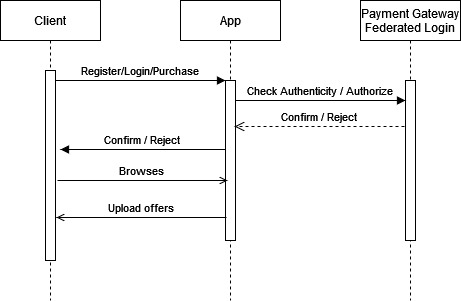
\includegraphics[width=0.7\textwidth]{assets/sequence_login_payment.jpg}
    \caption{Sequence of actions with 3rd party applications}
    \label{fig:sequence_login_payment}
\end{figure}

\subsubsection{Payment Gateway}

The usage of \gls{mobile payment gateway} offers three possibilities \cite{refonline:ZOPG}:

\begin{itemize}
    \item Redirection to payment processor's page
    \item Payment data and processing inside the application
    \item Payment data entered in the app, but processed with an \acrshort{api}
\end{itemize}

The third option stays in direct contact with our top quality attribute, usability. Since we want to offer a easy shopping
experience, the payment process should also be harmonic with other features.

\begin{table}[H]
    \setstretch{1.0}
    \begin{tabularx}{\textwidth}{|c|c|X|c|}
        \toprule
        \multicolumn{1}{c}{Tactict} & \multicolumn{1}{c}{Pattern} & \multicolumn{1}{c}{Motivation} & \multicolumn{1}{c}{QA} \\
        \midrule
        \textbf{Limit Dependencies} & \Gls{wrapper} & The \gls{api} will be the intermediary for the payment process. For the 
        \glsplural{client} all visible steps will occur in the app, without being sent to another page. On the background
        the \gls{api} will receive the input and send it to the payment gateway. The verification takes place in gateway, 
        which then communicate with the financial institute of the client and send the payment to the \gls{provider} 
        \cite{refonline:ZOPG}. & QA-2 \\
        \bottomrule
    \end{tabularx}
\end{table}

\subsubsection{Federated Authentication}

Using of \gls{federated login} reduces burden of saving user credentials locally. It also improves the Usability so users
do not have to create and remember another username and password. The authentication process takes place on the third 
party operator, as seen in the picture \ref{fig:sequence_login_payment}. 

\begin{table}[H]
    \setstretch{1.0}
    \begin{tabularx}{\textwidth}{|c|c|X|c|}
        \toprule
        \multicolumn{1}{c}{Tactict} & \multicolumn{1}{c}{Pattern} & \multicolumn{1}{c}{Motivation} \\
        \midrule
        \textbf{\gls{microservice}} & \gls{API Gateway} & It increases security, so the microservice is not directly
        exposed to the external world. It reduces the complexity of the microservice, since the gateway will have to deal
        with data transfer rate, tokens and other activities. Dealing with failures would also be handled and logged
        by the microservice \cite{refonline:javtop}. & QA-2\\
        \bottomrule
    \end{tabularx}
\end{table}

\subsection{Solution for Performance}

We want our app to have a fast (no more than 1 second) response time. By clicking on an offer a \gls{client} should
have it immediately displayed on his screen. Updated made by \glsplural{provider} should also be promptly available
for \glsplural{client} to browse.

\begin{table}[H]
    \setstretch{1.0}
    \begin{tabularx}{\textwidth}{|c|c|X|c|}
        \toprule
        \multicolumn{1}{c}{Tactict} & \multicolumn{1}{c}{Pattern} & \multicolumn{1}{c}{Motivation} & \multicolumn{1}{c}{QA} \\
        \midrule
        \textbf{Increase Resources} & \gls{Load Balancer} & Specially during peak times we want our users to have a 
        smoothly and fast interaction with the app. \Glsplural{provider} and \glsplural{client} should perform their
        tasks, either browsing, purchasing or uploading offering without having to wait to get a response. With this
        decision all requests would be forwarded to the server that are available avoiding queuing of requests. & QA-3 \\
        \bottomrule
    \end{tabularx}
\end{table}

\newpage

\subsection{Solution for Security}

There are two security concerns that need to be addressed to the users. The first one deals with the authentication
and payment process. This will be managed by the third party providers. The second one involves the interaction of
the \glsplural{provider} with the app. Since this stakeholder can upload data and file to the app it is important
that only approved data type is inserted. In the table below we will describe the tactics used for the these
two concerns.

% \begin{table}[H]
%     \setstretch{1.0}
%     \begin{tabularx}{\textwidth}{|c|c|X|c|}
%         \toprule
%         \multicolumn{1}{c}{Tactict} & \multicolumn{1}{c}{Pattern} & \multicolumn{1}{c}{Motivation} & \multicolumn{1}{c}{QA}\\
%         \midrule
%         \textbf{Validate Input} & \gls{Intercepting Validator} & \glsplural{provider} has a big interaction with the app.
%         They can upload files and texts. To make sure that only secure element a inserted into the app, it is important
%         that every input is analyzed before reaching the app and the \glsplural{client} \cite{refbook:CSWT}. & \multirow{3}{*}{QA-4} \\
%         \shortstack{\textbf{Authenticate Actors} \\ \textbf{Authorize Actors}} & \shortstack{Authentication enforcer\\
%         Authorization enforcer} & To avoid the connection of \gls{bots} we want to allow only registered users to interact with the functionalities 
%         of the app. This will be done with the third party operators \cite{refonline:wksp}. & QA-4\\
%         \bottomrule
%     \end{tabularx}
% \end{table}

\begin{table}[H]
    \setstretch{1.0}
    \begin{tabularx}{\textwidth}{|c|c|X|c|}
    \toprule
    \multicolumn{1}{c}{Tactict} & \multicolumn{1}{c}{Pattern} & \multicolumn{1}{c}{Motivation} & \multicolumn{1}{c}{QA} \\
    \midrule
    \multicolumn{1}{|c|}{\multirow{2}{*}{Support User Initiative}} & Observer & The interaction of the users is a main factor
    of our app. We want them to have fully control of their actions either by cancelling or by resuming an action.
    & \multirow{3}{*}{QA-4} \\
    \multicolumn{1}{|c|}{} & Lazy Registration & Avoid having to memorize another password and username may increase 
    the acceptance of the user. With this pattern we allow them also to browse in the app and seeing what is available 
    without being registered \cite{refonline:IDUI}. This may give a glimpse of what they get if they join us. &   \\

    Support System Initiative & Observer & By each upload from the \glsplural{provider} we want our \glsplural{client} 
    to have it on his device, without having to "ask" for it.  &  \\ 
    \bottomrule
    \end{tabularx}
\end{table}
